\section{Genetic Algorithms}
In this section we begin with a brief overview of the standard implementation of a Genetic Algorithm (GA) and include
pseudocode for the readers reference. Next, we discuss our implementation and the design choices made so we could easily
use our implementation for two different problems. We then look at one of these problems and highlight how a GA is an
appropriate choice. This also serves to provide the reader with an example of how a GA can be applied in practice.
Finally, we discuss the challenges faced in using the GA to solve this particular problem.


\subsection{Overview, Design and Intention}
Algorithm \ref{GA_alg} is our implementation of the standard GA. For a background please see [CITE]. Methods such as \textbf{SelectParent()}, \textbf{CrossOver()}, \textbf{Mutate()} and \textbf{CalculateFitness()} are abstract and implemented by the subclass.
In doing this, it was trivial to use the GA for two different problems. Additionally, it allowed us to experiment with 
different selection methods, such as proportional roulette, tournament and ranked roulette [CITE PAPER] by simply 
overriding \textbf{SelectParent()}. Similarly, the same can be said for crossover and mutation.
\begin{algorithm}[h]
\begin{algorithmic}
\State $children \gets$ InitEmptyPopulation()
\State $numChildren \gets 0$ 
\ForAll{$members$ in $population$} 
	\State $fitness[member] \gets$ CalculateFitness($member$)
\EndFor

\While{$numChildren < populationSize$}
	\State $parent1 \gets$ SelectParent()
	\State $parent2 \gets$ SelectParent()
	\If{$randomVal < crossoverRate$}
		\State $child1$, $child2 \gets $ CrossOver($parent1$, $parent2$)
	\Else
		\State $child1$, $child2 \gets $ Copy($parent1$, $parent2$)
	\EndIf
	\State Mutate($child1$) \Comment{\parbox[t]{.75\linewidth}{Where the mutate method handles which genes of the 
	chromosome get mutated according to the mutation rate.}}
	\State Mutate($child2$) 
	\State $children \gets children + child1$
	\State $children \gets children + child2$
	\State $numChildren \gets numChildren + 2$
\EndWhile
\State $population \gets children$ 
\caption{A standard Genetic Algorithm}
\label{GA_alg}
\end{algorithmic}
\end{algorithm}

We employ the use of GA's in our work and believe they are strongly applicable for the following reasons:
\begin{itemize}
\item Many solutions exist in the state space which would be infeasible to manually explore. By defining a fitness function
which encapsulates the properties of a desired solution, we can explore far more possibilities.
\item We can observe solutions which we may never have previously considered.
\item A GA framework is extensible and allows code reuse as the core algorithm can be used for different problems with 
minor changes.
\end{itemize}

\subsection{Tree Placement}
For a player to maximize the amount of resources they collect, a certain subsection of the map
may be far more profitable than another. However, in order to know this they must discover it. If the map topology
remained static, the player would always head to the most profitable area without much pause for thought.
In order to make subsequent games more interesting and enjoyable, we decided to randomize the placement of
the resource trees. 
\begin{figure}[h]
        \centering
        \begin{subfigure}[b]{0.482\linewidth}
                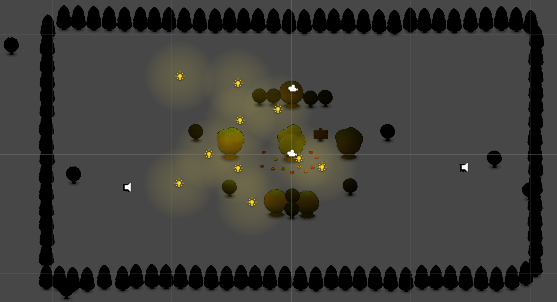
\includegraphics[width=\linewidth]{./ga_n1}
                \caption{}
                \label{fig:ga_step1}
        \end{subfigure}
        \begin{subfigure}[b]{0.49\linewidth}
                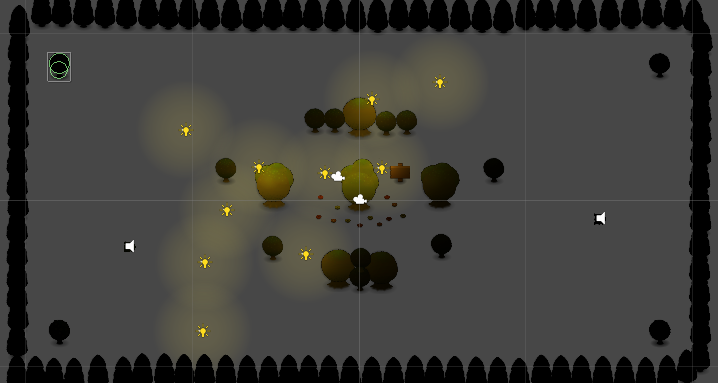
\includegraphics[width=\linewidth]{./ga_n2}
                \caption{}
                \label{fig:ga_step2}
        \end{subfigure}
        \begin{subfigure}[b]{0.5\linewidth}
                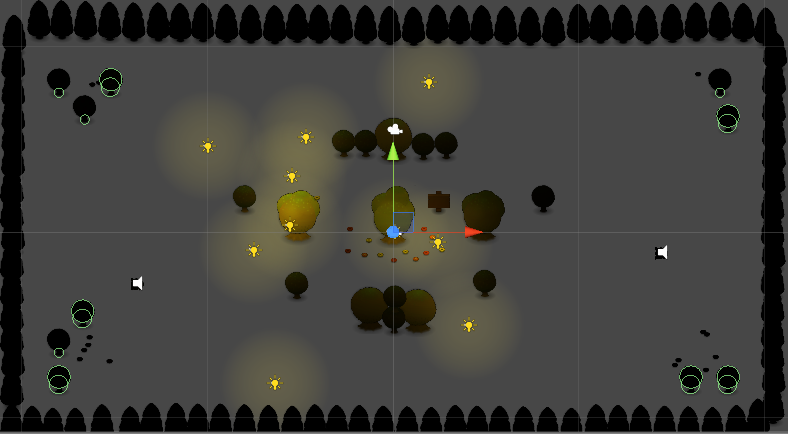
\includegraphics[width=\linewidth]{./ga_n3}
                \caption{}
                \label{fig:ga_step3}
        \end{subfigure}
        \begin{subfigure}[b]{0.49\linewidth}
               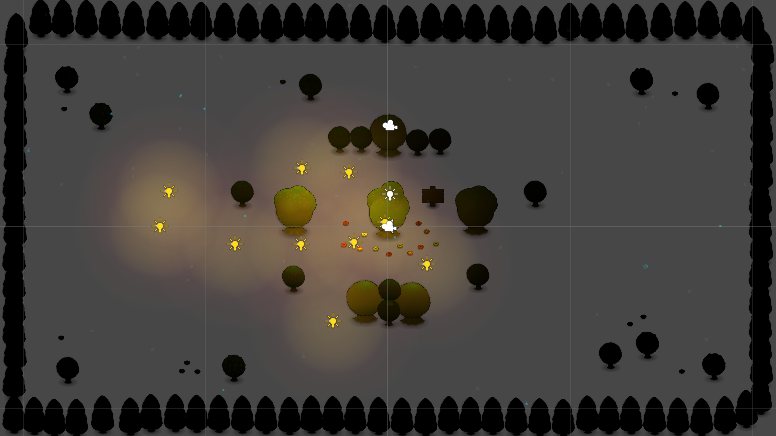
\includegraphics[width=\linewidth]{./ga_final}
           	   \caption{}
               \label{fig:ga_step4}
        \end{subfigure}
        \caption{The steps to implementing an appropriate fitness function. In \ref{fig:ga_step1} the trees are placed 
        outside of the game border. If we left the GA to run for 100,000 iterations, the trees were much further away and 
        to see them the scene must be zoomed out. In \ref{fig:ga_step2} we remedied this problem , yet created a new one. 
        Here the trees remained in the four corners of the map as the GA found an optimal solution which maximised this 
        fitness function. To prevent this behaviour, we simply run for less generations. Figure \ref{fig:ga_step3} shows 
        the inclusion of flower positions. As one can see there is quite a lot which are clustered. Removing the number of flowers generated did not solve this issue. Instead, the fitness function needed to be clarified. Figure 
        \ref{fig:ga_step4} shows the final fitness function and GA parameter set. Here the flowers and trees are spread out 
        far more. Additionally, this iteration of the GA gives a better amount of randomization on subsequent 
        runs.}
        \label{fig:GA_Trees}
\end{figure}


\subsection{Challenges}
In this section we highlight the challenges we faced for the specific problem of randomizing
the placement of objects in the game world. We leave discussion of the challenges related to evolving weights
for a neural net to train a frog controller for section \ref{sec:neural}.
\subsubsection{Succint Fitness Function}
\subsubsection{Generating Positions at Runtime}


\subsection{Outcome}
Figure \ref{fig:ga_outcome} shows three different solutions generated by the final fitness functions and parameter set.
It's interesting to note the variations in each.
\begin{figure}[h]
        \centering
        \begin{subfigure}[b]{0.48\linewidth}
                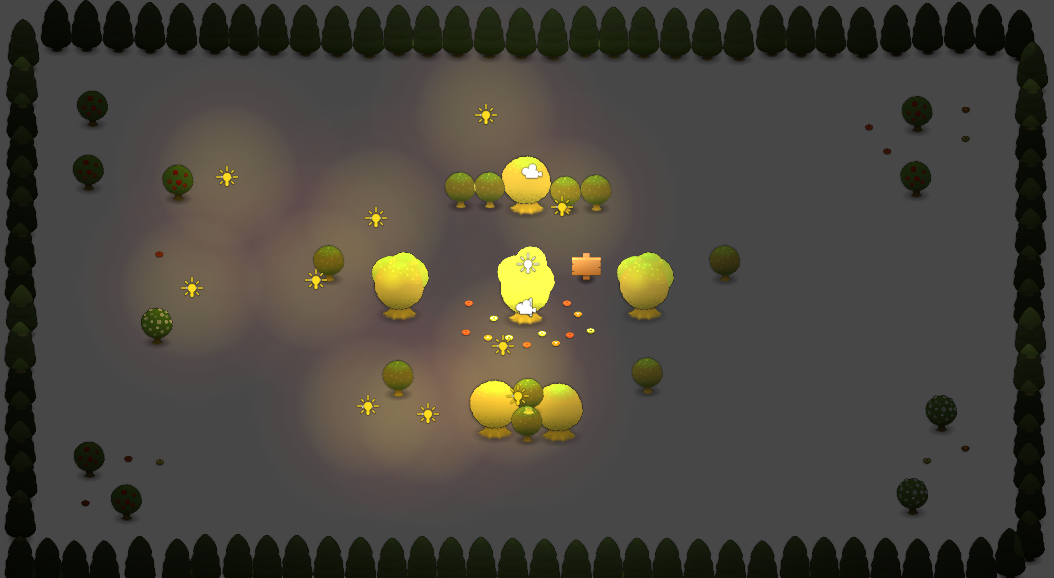
\includegraphics[width=\linewidth]{./ga_outcome_1}
                \caption{}
                \label{fig:ga_outcome_1}
        \end{subfigure}
        \begin{subfigure}[b]{0.48\linewidth}
                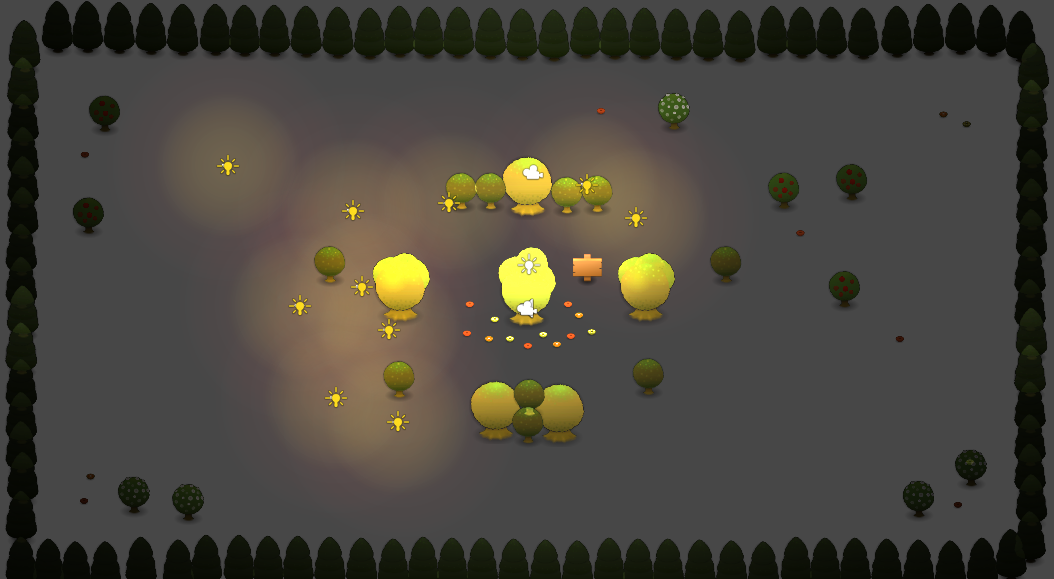
\includegraphics[width=\linewidth]{./ga_outcome_2}
                \caption{}
                \label{fig:ga_outcome_2}
        \end{subfigure}
        \begin{subfigure}[b]{0.48\linewidth}
                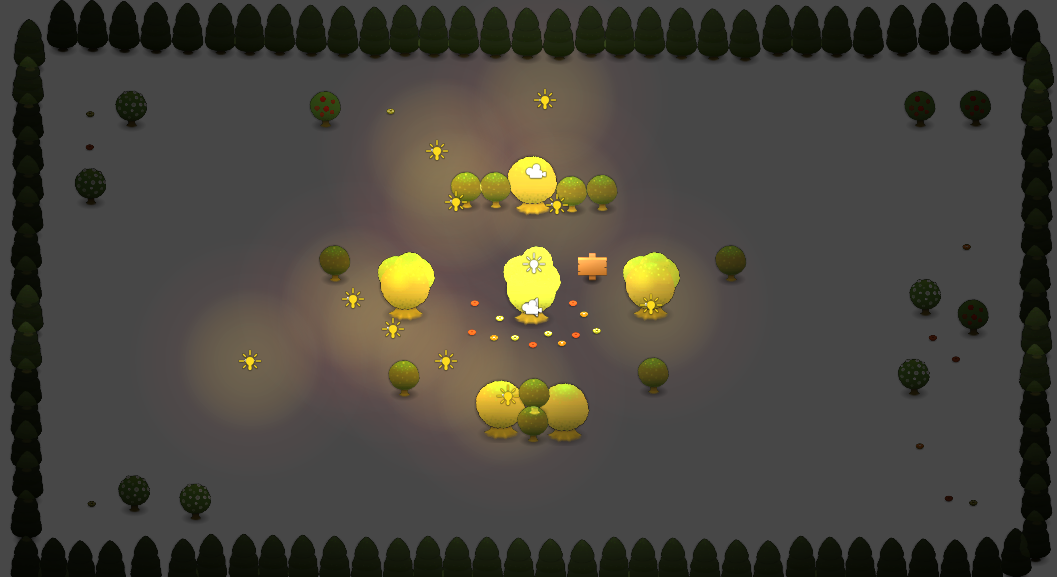
\includegraphics[width=\linewidth]{./ga_outcome_3}
                \caption{}
                \label{fig:ga_outcome_3}
        \end{subfigure}
        \begin{subfigure}[b]{0.48\linewidth}
                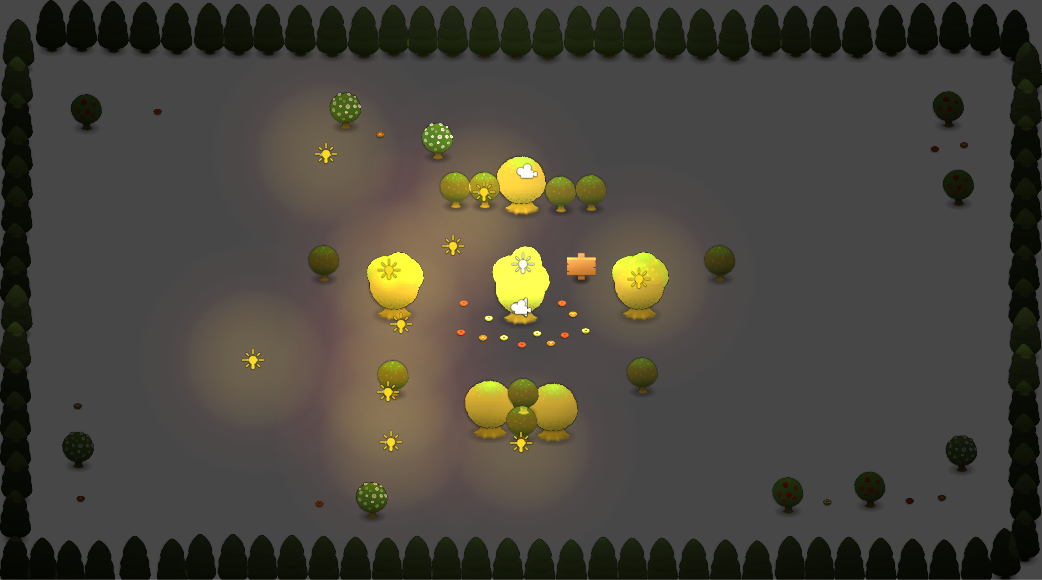
\includegraphics[width=\linewidth]{./ga_outcome_4}
                \caption{}
                \label{fig:ga_outcome_4}
        \end{subfigure}
        \begin{subfigure}[b]{0.48\linewidth}
                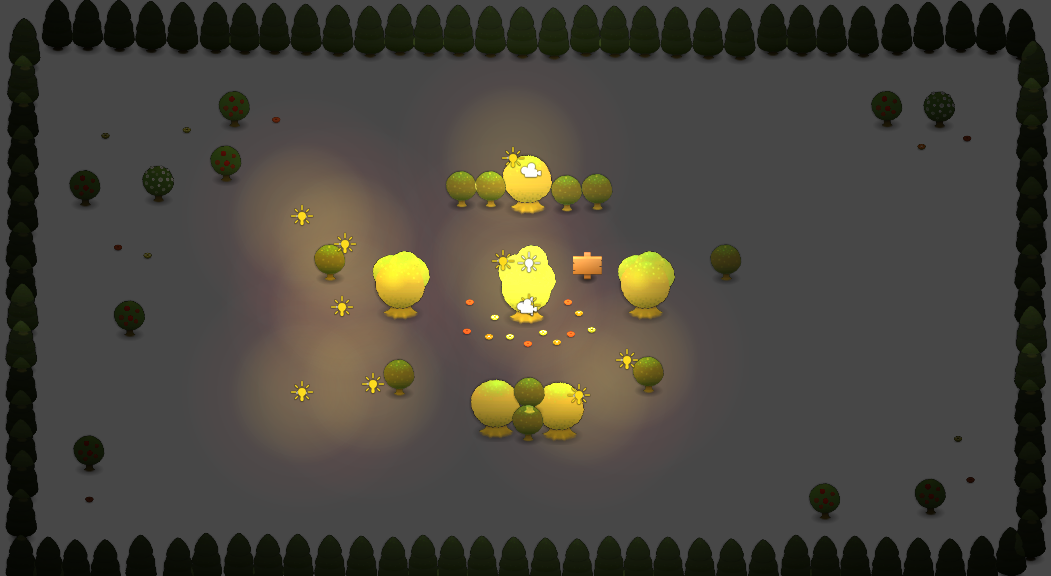
\includegraphics[width=\linewidth]{./ga_outcome_5}
                \caption{}
                \label{fig:ga_outcome_5}
        \end{subfigure}
        \begin{subfigure}[b]{0.48\linewidth}
                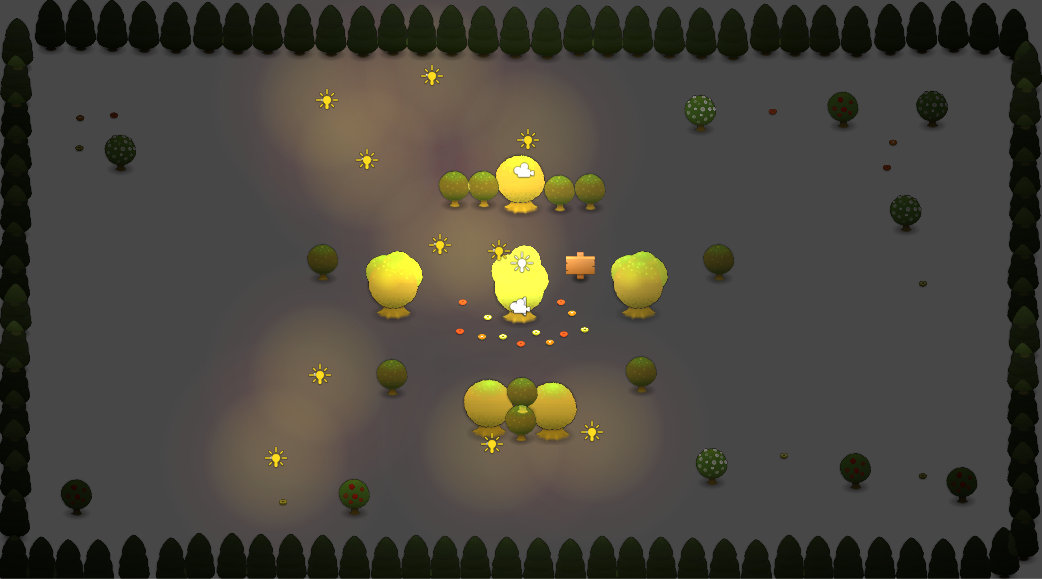
\includegraphics[width=\linewidth]{./ga_outcome_6}
                \caption{}
                \label{fig:ga_outcome_6}
        \end{subfigure}
        \caption{}
        \label{fig:GA_Final}
\end{figure}